\chapter{Methodik}
\label{ch:methodik}
\todo{deutlich machen, was ich anders gemacht habe als Pawara und wieso}
\todo{generelles Verfahren in eigenen Worten beschreiben}

\section{OvO-Kodierung}
\label{ch:methodik_kodierung}
\todo{Umsetzung: OvO Matrix, Kodierung, Klassifizierung, eigene Loss-Funktion, softmax vs tanh}
\todo{Warum Datensätze mit 3 Klassen verwendet wurden}

\subsection{Alternative Kodierungsmethoden}
\todo{alternative Kodierungsmöglichkeiten beschreiben (s. Paper, z.B. Error correcting codes)}

\newpage
\section{Datensätze}
\label{ch:methodik_datensaetze}
Für die Experimente wurden 5 verschiedene Datensätze verwendet: Agrilplant \cite{pawaraWebsiteDatensaetze}, Cifar \cite{cifar10}, Monkey \cite{pawaraWebsiteDatensaetze}, SwedishLeaves \cite{swedishLeaves} und Tropic \cite{pawaraWebsiteDatensaetze}.

Für jeden Datensatz existieren Exemplare mit verschiedenen Anzahlen an Klassen (s. Abb. \ref{fig:DatensatzKlassen}), die zukünftig jeweils mit $<$Datensatzname$><$Klassenanzahl$>$ wie z.B. Agrilplant10 bezeichnet werden.
Die Datensätze mit geringerer Klassenanzahl sind Teilmengen des gesamten Datensatzes, bei denen nur die ersten $k$ Klassen verwendet werden.

Bei allen Datensätzen außer SwedishLeaves (s. Kapitel \ref{ch:methodik_SwedishLeaves}) wird eine 5-Fold Cross Validation angewendet, es werden also 5 Aufteilungen in Train- und Testdaten im Verhältnis 80:20 erstellt, sodass sich jedes Bild genau in einem Fold im Testsplit und in 4 Folds im Trainsplit befindet.

Für die Datensätze Tropic10 und Monkey10 stehen auf der Homepage der Autorin \cite{pawaraWebsiteDatensaetze} die von ihr verwendeten Einteilungen in 5 Folds zur Verfügung. Diese Datensätze, die mit der exakt gleichen Einteilung in 5 Folds verwendet wurden, werden im weiteren Verlauf dieser Arbeit mit dem Präfix\\ \enquote{Pawara-} kenntlich gemacht. Da die gleiche Einteilung in 5 Folds verwendet wurde wie im Paper von Pawara et al. \cite{pawaraPaper} ist die Vergleichbarkeit der reproduzierten Ergebnisse höher.

Für alle anderen Datensätze musste die Einteilung in 5 bzw. für SwedishLeaves 3 Folds neu erstellt werden.
Außerdem wurde für Tropic10 ebenfalls eine eigene 5-Fold Cross Validation erstellt, da die von der Autorin zur Verfügung gestellte Einteilung (s. \cite{pawaraWebsiteDatensaetze}) fehlerhaft ist. Ihre sogenannte 5-Fold Cross Validation besteht bei Tropic10 vermutlich aus fünfmaligem, zufälligem Ziehen eines Verhältnisses 70:30 für Trainings und Testdaten. Dies führt dazu, dass ein eventuell schwierig zu klassifizierendes Bild in mehr als einem Fold im Testsplit vorkommen und somit das Ergebnis abhängig vom Zufall beeinflussen kann.
\todo{In Scatterplots schauen, inwiefern diese Aussage stimmt}

\begin{figure}[H]
\begin{tabular}{|c|c|c|c|c|c|}
\hline 
Anzahl an Klassen & 3 & 5 & 10 & 15 & 20 \\ 
\hline 
Agrilplant & X & X & X &  &  \\ 
Cifar &  &  & X &  &  \\ 
Monkey &  &  & X &  &  \\ 
SwedishLeaves & X & X & X & X &  \\ 
Tropic & X & X & X & & X \\ 
\hline 
\end{tabular} 
\caption{Zum Training verwendete Anzahl an Klassen je Datensatz}
\label{fig:DatensatzKlassen}
\end{figure}

\subsection{Agrilplant}
Der Agrilplant Datensatz \cite{pawaraWebsiteDatensaetze} besteht aus Bildern von Blüten, Früchten und Blättern von Agrarpflanzen.
Es existieren 10 verschiedene Klassen: Apfel, Banane, Traube, Jackfruit, Orange, Papaya, Kaki, Ananas, Sonnenblume und Tulpe (vgl. \cite{pawaraWebsiteDatensaetze}).
\begin{figure}[H]
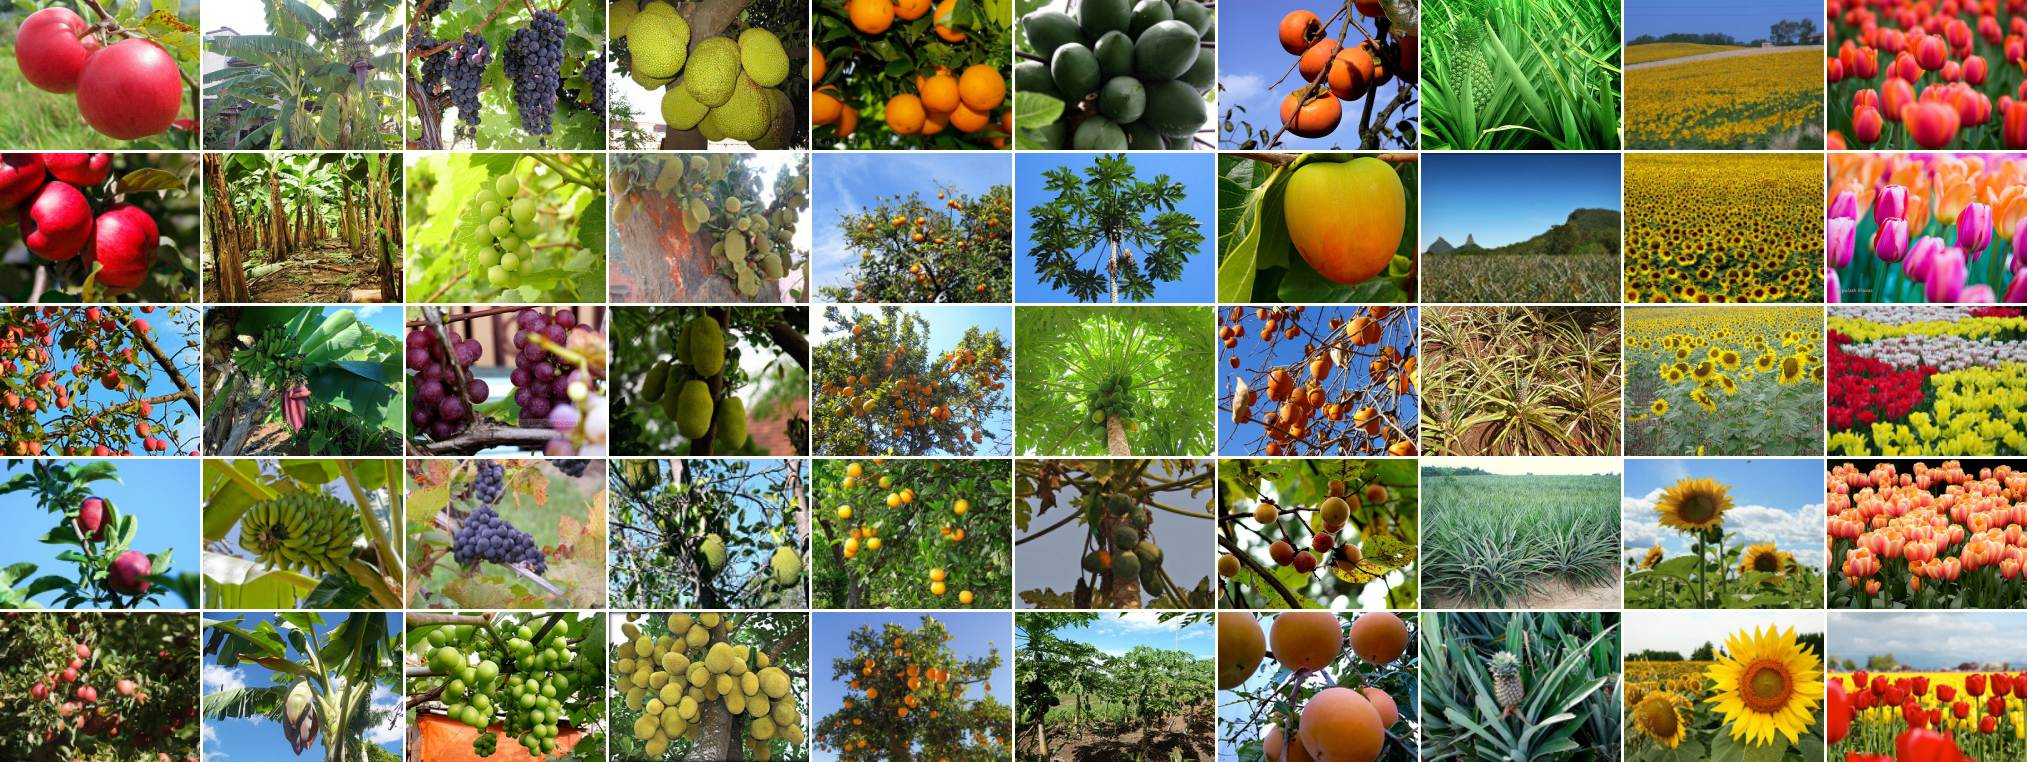
\includegraphics[scale=0.2]{img/2_agrilplant-image.jpg}
\caption{Überblick über die verschiedenen Klassen des Agrilplant Datensatzes \cite{pawaraAgrilplant}.}
\label{fig:agrilplantUeberblick}
\end{figure}

Zum Training wurden zusätzlich zu Agrilplant10 noch zwei weitere Teilmengen des Datensatzes, Agrilplant5 und Agrilplant3, verwendet.

Der Datensatz Agrilplant10 besteht aus 300 Bildern mit einer Auflösung von ca. 200-500 Pixeln je Klasse, also insgesamt 3000 Bilder, und ist damit perfekt ausbalanciert (s. Abb. \ref{fig:Agrilplant10Zusammensetzung}).\\


\begin{figure}[H]
\begin{adjustbox}{width=1.4\textwidth, center}
\includesvg{img/2_agrilplant10_Zusammensetzung}
\end{adjustbox}
\caption{Aufteilung des Agrilplant10 Datensatzes \cite{pawaraWebsiteDatensaetze} in Train- und Testsplits je Fold.}
\label{fig:Agrilplant10Zusammensetzung}
\end{figure}


\subsection{Cifar}
Der Cifar10 Datensatz beinhaltet insgesamt 60.000 Bilder in einer sehr kleinen Auflösung von 32x32 Pixeln. Es existieren 10 Klassen: Flugzeug, Automobil, Vogel, Katze, Hirsch, Hund, Frosch, Pferd, Schiff, Lastkraftwagen (vgl. \cite{cifar10}).
Die Aufteilung in Klassen ist perfekt ausbalanciert mit genau 6.000 Bildern pro Klasse (s. Abb. \ref{fig:Cifar10Zusammensetzung}).
Da die zum Training verwendeten Netze für Bilder in einer Auflösung von 224 bzw. 299 Pixeln ausgelegt sind (vgl. \ref{ch:methodik_netze}) müssen die Bilder von diesem Datensatz ungefähr 8-fach vergrößert werden.\\

Durch die große Anzahl an Bildern und die starke Hochskalierung benötigt das Training viel Zeit und Ressourcen, weshalb Cifar10 nur bei Resnet Scratch verwendet wird.
\todo{Verlinkung setzen auf Trainingsdauer, Aussage wie viel länger als z.B. Tropic20}

Dieser Datensatz wurde zusätzlich zu den anderen ausgewählt um die Aussagekraft der Ergebnisse zu erhöhen, da sich die anderen Datensätze lediglich auf Pflanzen und Affen beschränken. Im wissenschaftlichen Paper von Pawara et al. \cite{pawaraPaper} wird dieser Datensatz nicht behandelt.

\begin{figure}[H]
\begin{adjustbox}{width=1.4\textwidth, center}
\includesvg{img/2_cifar10_Zusammensetzung}
\end{adjustbox}
\caption{Aufteilung des Cifar10 Datensatzes \cite{cifar10} in Train- und Testsplits je Fold.}
\label{fig:Cifar10Zusammensetzung}
\end{figure}


\subsection{Monkey}
Für den Monkey Datensatz existieren 2 Versionen: Pawara-Monkey10 und Pawara-uMonkey10 mit absichtlich nicht ausbalancierten Anzahlen an Bildern je Klasse, um zu untersuchen wie die beiden Klassifikationsschemata auf schlecht ausbalancierten Datensätzen abschneiden (vgl. \cite{pawaraWebsiteDatensaetze}). Beide Versionen bestehen aus Bildern aus 10 Klassen von verschiedenen Affenarten aufgenommen in freier Wildbahn aus unterschiedlichen Perspektiven (s. Abb. \ref{fig:monkey10Ueberblick}) und wurden in genau der gleichen Aufteilung in Folds bei den Experimenten im Paper von Pawara et al. \cite{pawaraPaper} verwendet.
Die Bilder haben eine Auflösung von ca. 180 bis zu 6.000 Pixeln.
\begin{figure}[H]
\centering
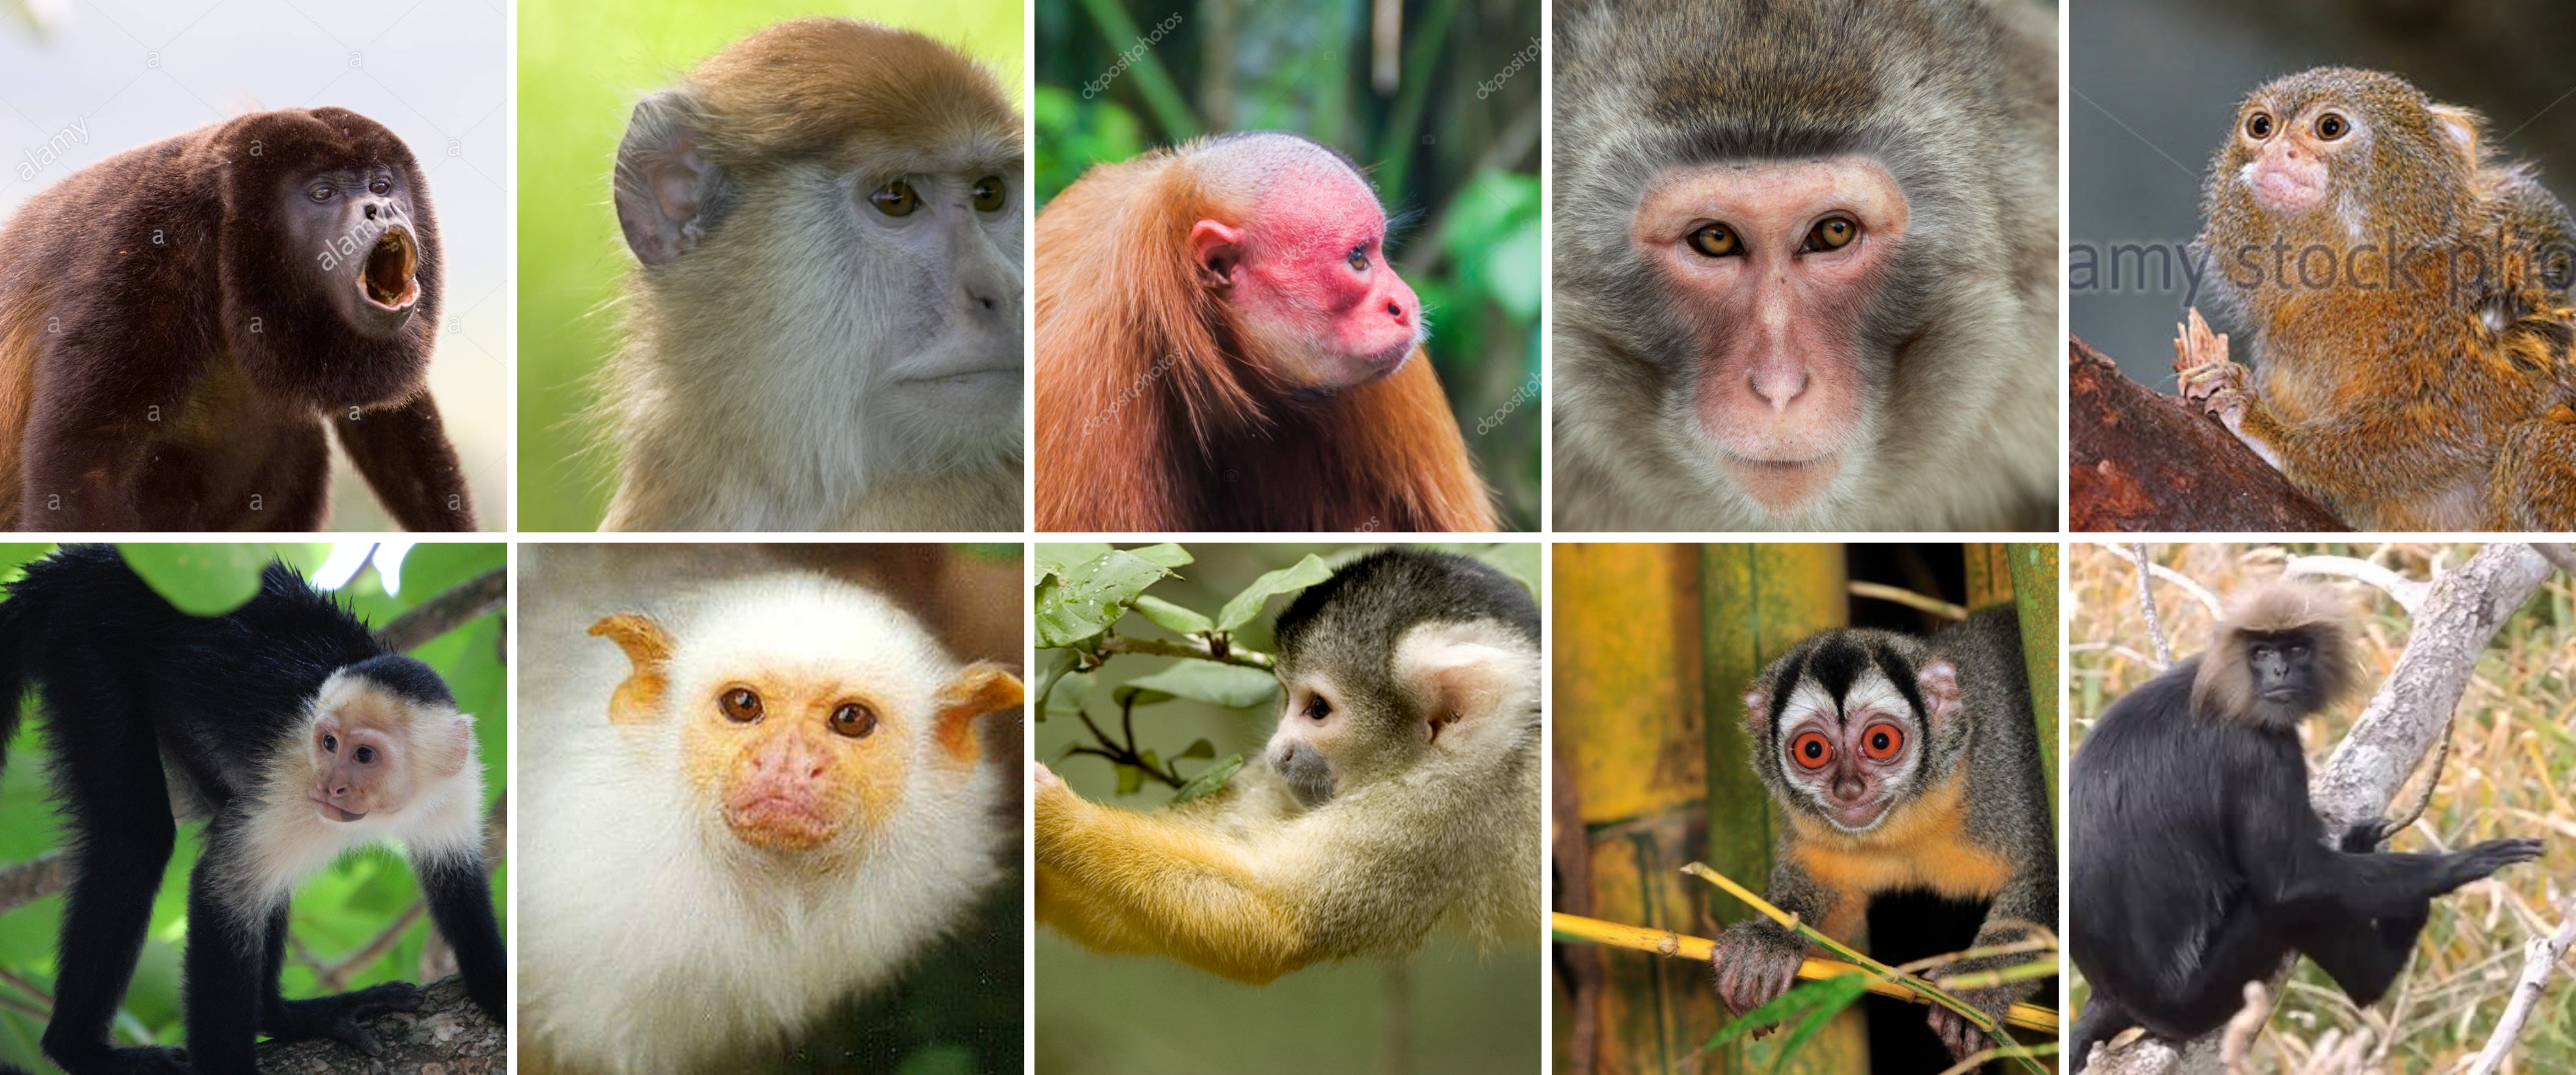
\includegraphics[scale=0.08]{img/2_monkey10-image.jpg}
\caption{Überblick über die verschiedenen Klassen des Monkey10 Datensatzes \cite{pawaraMonkey}.}
\label{fig:monkeyUeberblick}
\end{figure}

Der Pawara-Monkey10 Datensatz besteht aus insgesamt 1370 Bildern und ist mit 131 bis 152 Bildern je Klasse noch relativ gut ausbalanciert (s. Abb \ref{fig:Pawara-Monkey10Zusammensetzung}).\\

Im Gegensatz dazu ist der Datensatz Pawara-uMonkey10 weder in der Anzahl an Bildern pro Klasse noch in der Größe der Folds im Trainsplit ausbalanciert (s. Abb. \ref{fig:Pawara-uMonkey10Zusammensetzung}). 


\begin{figure}[H]
\begin{adjustbox}{width=1.4\textwidth, center}
\includesvg{img/2_pawara-monkey10_Zusammensetzung}
\end{adjustbox}
\caption{Aufteilung des Pawara-Monkey10 Datensatzes \cite{pawaraWebsiteDatensaetze} in Train- und Testsplits je Fold.}
\label{fig:Pawara-Monkey10Zusammensetzung}
\end{figure}
\begin{figure}[H]
\begin{adjustbox}{width=1.4\textwidth, center}
\includesvg{img/2_pawara-umonkey10_Zusammensetzung}
\end{adjustbox}
\caption{Aufteilung des unbalancierten Pawara-uMonkey10 Datensatzes \cite{pawaraWebsiteDatensaetze} in Train- und Testsplits je Fold.}
\label{fig:Pawara-uMonkey10Zusammensetzung}
\end{figure}





\subsection{SwedishLeaves}
\label{ch:methodik_SwedishLeaves}
Der SwedishLeaves Datensatz besteht aus Bildern von Blättern schwedischer Bäume, die zentriert auf einem weißen Hintergrund liegen (s. Abb. \ref{fig:swedishLeavesUeberblick}). Dadurch besitzen Bilder innerhalb einer Klasse eine hohe Ähnlichkeit.

\begin{figure}[H]
\centering
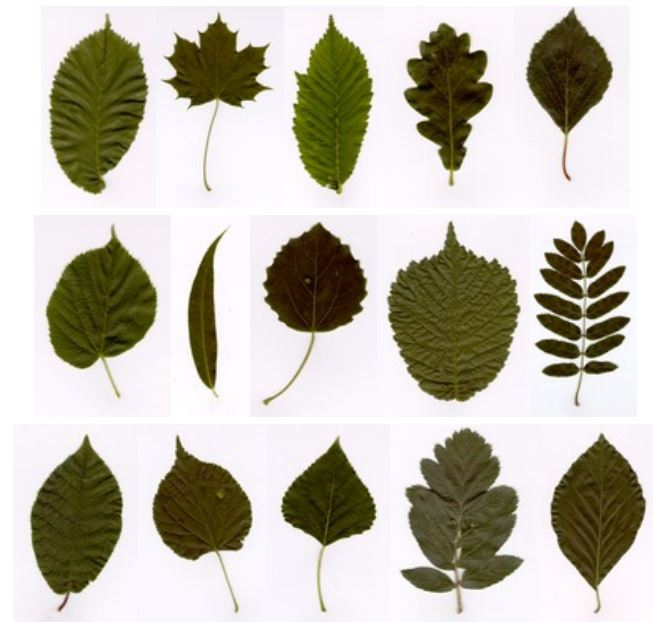
\includegraphics[scale=0.8]{img/2_swedishLeaves-image.jpg}
\caption{Überblick über die verschiedenen Klassen des SwedishLeaf Datensatzes \cite{pawaraMonkey}.}
\label{fig:swedishLeavesUeberblick}
\end{figure}

In den Experimenten von Pawara et al. \cite{pawaraPaper} wurde fünfmal ein Verhältnis von 1:2 für Trainings- und Testdaten aus den 75 Bildern pro Klasse gezogen (vgl. \cite{pawaraPaper} Kapitel 3.1.3), sodass im Testsplit doppelt so viele Bilder sind wie im Trainsplit.

Da hierbei offensichtlich Doppelungen zwischen den Folds entstehen und die verwendete Einteilung der Autorin des Papers \cite{pawaraPaper} nicht verfügbar ist, habe ich mich dafür entschieden die 75 Bilder pro Klasse in 3 Gruppen zu je 25 Bildern auf zu teilen und daraus 3 Folds mit einem Verhältnis von 1:2 für Trainings und Testdaten zu mischen. Dabei gelangt jedes Bild genau in einem Fold in den Trainsplit und in zwei Folds in den Testsplit. Es entsteht quasi eine 3-Fold Cross Validation mit vertauschtem Train- und Testsplit (s. Abb. \ref{fig:swedishLeavesZusammensetzung}).

Zusätzlich zu SwedishLeaves15 wurde mit drei weiteren Teilmengen des Datensatzes gearbeitet: SwedishLeaves10, SwedishLeaves5 und SwedishLeaves3.

\begin{figure}[H]
\begin{adjustbox}{width=1.4\textwidth, center}
\includesvg{img/2_swedishLeaves15_Zusammensetzung}
\end{adjustbox}
\caption{Aufteilung des SwedishLeaves15 Datensatzes \cite{swedishLeaves} in Train- und Testsplits je Fold.}
\label{fig:swedishLeavesZusammensetzung}
\end{figure}

\subsection{Tropic}
In dem Tropic Datensatz \cite{pawaraWebsiteDatensaetze} befinden sich 20 Klassen mit Bildern tropischer Pflanzen und deren Blättern, Blüten und Früchten (s. Abb. \ref{fig:tropicUeberblick}). Da unterschiedliche Teile der Pflanzen aus verschiedenen Blickwinkeln vor vielfältigen Hintergründen wie z.B. Erde, Himmel, Straßen oder Häusern fotografiert wurden ist die Klassifikation im Vergleich zum SwedishLeaves Datensatz \cite{swedishLeaves} (s. Kapitel \ref{ch:methodik_SwedishLeaves}) wesentlich anspruchsvoller.


\begin{figure}[H]
\centering
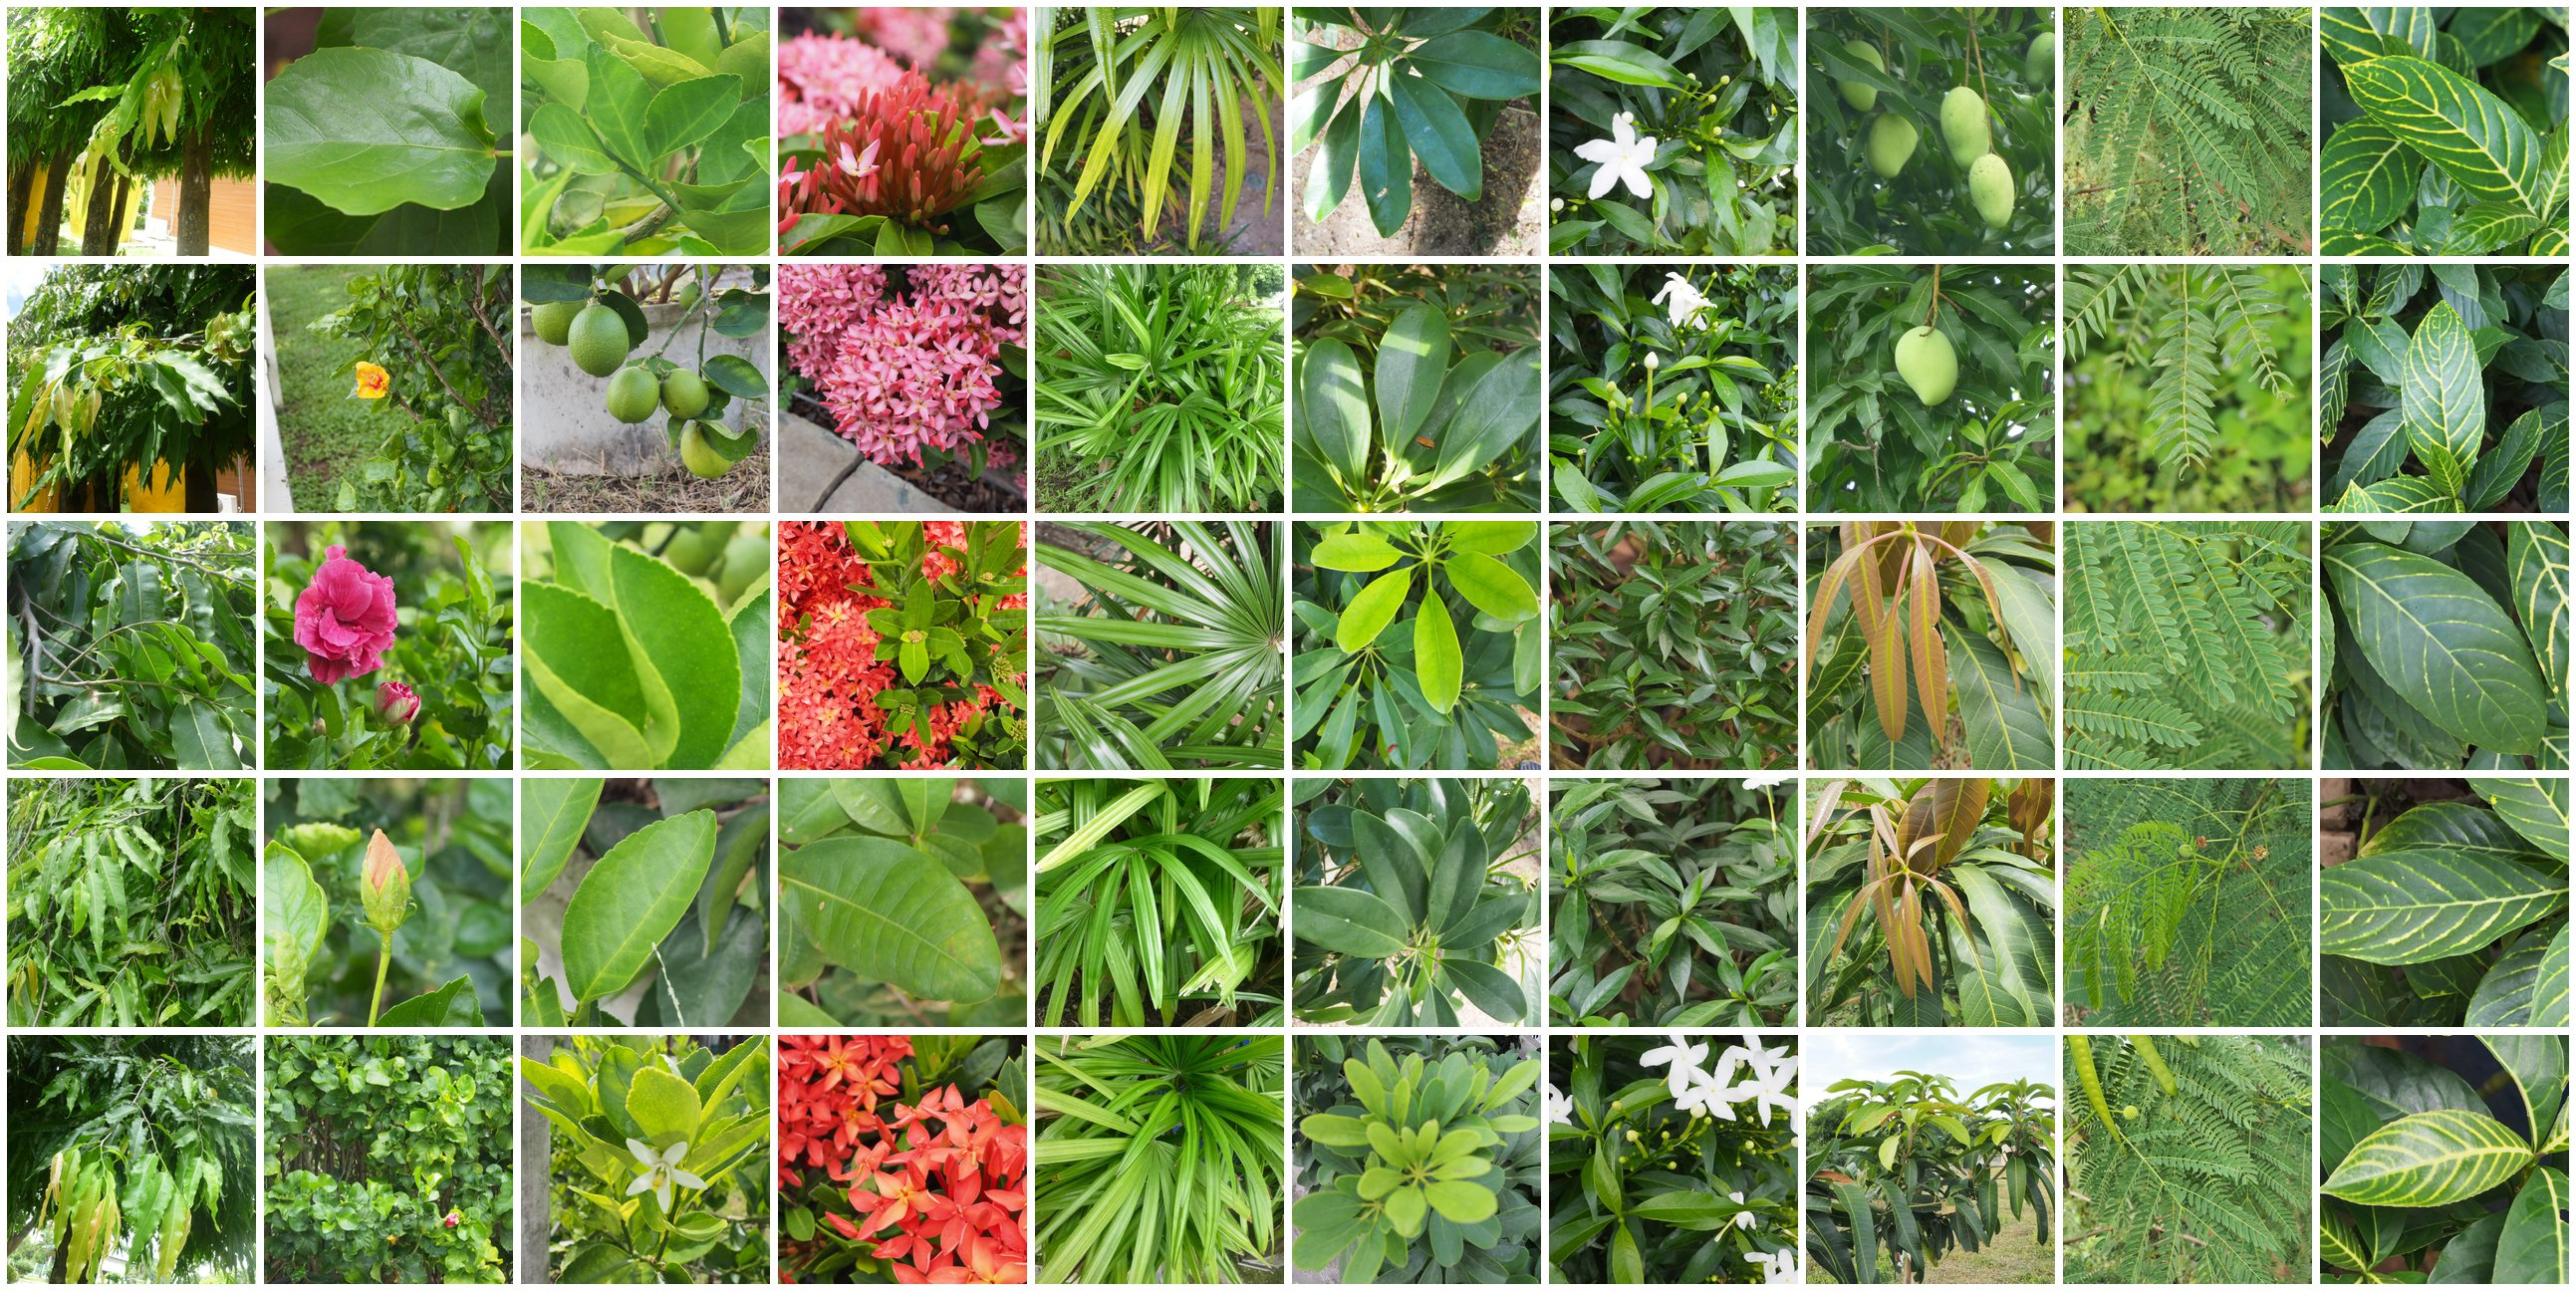
\includegraphics[scale=0.14]{img/2_tropic10-image.jpg}
\caption{Überblick über die verschiedenen Klassen des\\
Tropic Datensatzes \cite{pawaraTropic}.}
\label{fig:tropicUeberblick}
\end{figure}

Pro Klasse existieren 221-371 Bilder (s. Abb. \ref{fig:tropic20Zusammensetzung} und Abb. \ref{fig:pawaraTropic10Zusammensetzung}) in einer Auflösung von 250x250 Pixeln.

Es wurden Teilmengen von diesem Datensatz mit 20, 10, 5 und 3 Klassen zum Vergleich der beiden Klassifikationsschemata verwendet. Außerdem wurde die von Pawara et al. im Paper \cite{pawaraPaper} verwendete Einteilung in Folds \textit{Pawara-Tropic10} \cite{pawaraWebsiteDatensaetze} benutzt, bei der die 5-Fold Cross Validation aus fünfmaligem, zufälligem Ziehen eines Verhältnisses 70:30 für Trainings- und Testdaten besteht (s. Abb. \ref{fig:pawaraTropic10Zusammensetzung}).
Zusätzlich existiert noch ein Tropic52 Datensatz \cite{pawaraWebsiteDatensaetze} mit 52 Klassen, der aber weder im Paper von Pawara et al. \cite{pawaraPaper} noch in dieser Bachelorarbeit behandelt wird.

\begin{figure}[H]
\begin{adjustbox}{width=1.4\textwidth, center}
\includesvg{img/2_tropic20_Zusammensetzung}
\end{adjustbox}
\caption{Aufteilung des Tropic20 Datensatzes \cite{pawaraWebsiteDatensaetze} in Train- und Testsplits je Fold.}
\label{fig:tropic20Zusammensetzung}
\end{figure}
\begin{figure}[H]
\begin{adjustbox}{width=1.4\textwidth, center}
\includesvg{img/2_pawara-tropic10_Zusammensetzung}
\end{adjustbox}
\caption{Aufteilung des Pawara-Tropic10 Datensatzes \cite{pawaraWebsiteDatensaetze} in Train- und Testsplits je Fold.}
\label{fig:pawaraTropic10Zusammensetzung}
\end{figure}


\section{Trainingsparameter}
\label{ch:methodik_parameter}
Um zu untersuchen wie OvO und OvA im Vergleich zueinander in verschiedenen Situationen abschneiden, werden die folgenden Trainingsparameter für beide Klassifikationsschemata variiert.
Dadurch kann eine allgemeinere Aussage über die Vor- und Nachteile der OvO und OvA Klassifikation getroffen werden, da man durch die Variation der Trainingsparameter einen größeren Bereich an potentiellen Anwendungsfällen abdeckt.

Außerdem kann durch die verschiedenen Trainingsparameter analysiert werden, in welchen Situationen die OvO Klassifikation seine theoretischen Vorteile in der Praxis besonders gut ausnutzen kann und wann sich eine Implementation des OvO Klassifikationsschemas eher nicht lohnt.

\subsection{Frameworks}
Zu Beginn wurde das Training für diese Bachelorarbeit mit TensorFlow 2.4.1 \cite{tensorflow} durchgeführt. Jedoch wurde schnell deutlich, dass die Ergebnisse mit dieser Version von TensorFlow nicht den Erwartungen entsprechen und nicht mit den im Paper von Pawara et al. \cite{pawaraPaper} vorgestellten Ergebnissen übereinstimmen. Dabei sind die Abweichungen bei einigen Datensätzen und Kombinationen von Trainingsparametern deutlich größer als bei anderen (s. Kapitel \ref{ch:ergebnisse} und \ref{ch:diskussion}). \\

Die Autoren haben leider nicht angegeben, mit welcher Version von TensorFlow \cite{tensorflow} ihre Experimente durchgeführt wurden. Aber anhand des Veröffentlichungsdatums des Papers \cite{pawaraPaper} kann grob abgeschätzt werden, welche Version möglicherweise verwendet wurde.

Somit wurden zusätzlich die gleichen Experimente erneut mit der auf Palma II \cite{palma2} bereits vorinstallierten TensorFlow \cite{tensorflow} Version 1.13.1 durchgeführt.

Da zwischen diesen beiden Versionen von TensorFlow \cite{tensorflow} bereits erhebliche Diskrepanzen aufgetreten sind, wurden zum Schluss erneut die gleichen Experimente in PyTorch 1.9.0 \cite{pytorch} durchgeführt.
Damit soll sichergestellt werden, dass die Aussage über die Auswirkung der OvO oder OvA Klassifikation nicht nur auf bestimmte Versionen von TensorFlow \cite{tensorflow} zutrifft sondern möglichst allgemeingültig auf andere Machine-Learning Frameworks übertragen werden kann.

\todo{Implementation von Resnet und Inception vergleichen}

\subsection{Netztypen}
\label{ch:methodik_netze}
Für das Training werden die zwei beliebten Netzarchitekturen \textit{ResNet-50} und \textit{Inception V3} verwendet. Als Auflösung der Bilder für die Netze wurde bei \textit{ResNet-50} standardmäßig 224x224 Pixel und bei \textit{Inception V3} 299x299 Pixel verwendet. Größere oder kleinere Bilder in den Datensätzen wurden entsprechend skaliert.

Für das Netz \textit{Inception V3} hat die Autorin in dem auf Ihrer Webseite zur Verfügung gestellten Quellcode \cite{pawaraWebsiteCode} einige Änderungen an den letzten Schichten des Netzes vorgenommen. So wird beispielsweise eine zusätzliche \textit{BatchNormalization}-Schicht und eine \textit{Dropout}-Schicht eingefügt, die es in der Standardimplementierung von \textit{Inception V3} nicht gibt (s. Abb. \ref{fig:inceptionAenderungen}).

Die letzte Schicht, die \textit{Dense} oder \textit{Fully Connected} Schicht, wurde für OvO und OvA jeweils auf die entsprechende Anzahl an Klassifikatoren angepasst. Für die OvA Klassifikation hat das Netz genau so viele Ausgabewerte wie es Klassen gibt, für OvO gibt das Netz bei $k$ Klassen $\frac{k(k-1)}{2}$ Werte entsprechend des OvO Kodierungsschemas (s. Kapitel \ref{ch:methodik_kodierung}) aus.

\begin{figure}[H]

\begin{minipage}{.5\textwidth}
\begin{figure}[H]
\begin{adjustbox}{width=\textwidth, center}
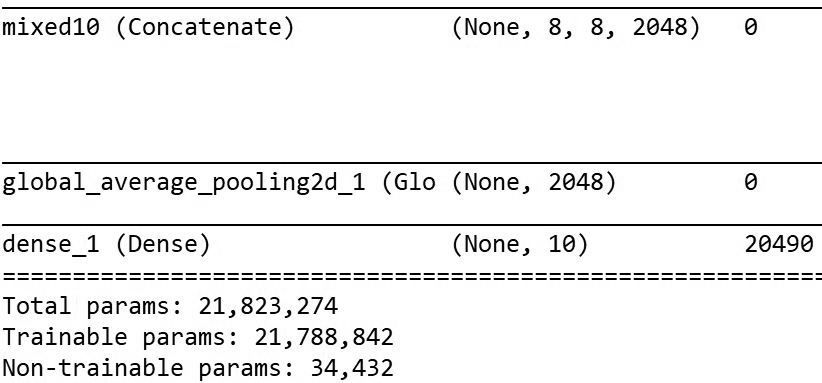
\includegraphics[scale=1]{img/3_inception-standard.jpg}
\end{adjustbox}
\end{figure}
\end{minipage}%
\begin{minipage}{.5\textwidth}
\begin{figure}[H]
\begin{adjustbox}{width=\textwidth, center}
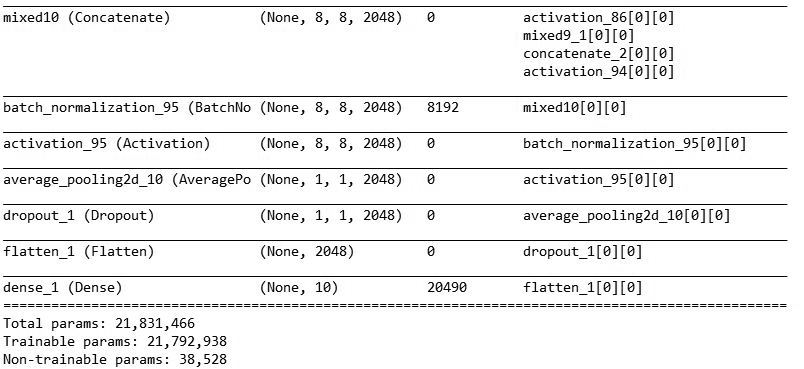
\includegraphics[scale=1]{img/3_inception-pawara.jpg}
\end{adjustbox}

\end{figure}
\end{minipage}
\caption{Standardmäßiger Aufbau des \textit{Inception V3} Netzes (links) und Änderungen an den letzten Schichten des \textit{Inception V3} Netzes von Pawara et al. \cite{pawaraWebsiteCode} (rechts).}
\label{fig:inceptionAenderungen}
\end{figure}


\subsection{Trainsize}

\todo{deterministische Datensatz-Splits}

\subsection{Klassenanzahl}

\subsection{vortrainierte Gewichte}
\todo{Epochen, Learningrate}


\section{Ausführung der Jobs auf Palma II}
\label{ch:methodik_palma}
\todo{Hardware auf Palma, Einteilung in Jobs, Logging, benutzte Grafikkarten, CPU Limits}

